%============================================================================
% PREÁMBULO
%============================================================================
\documentclass[letterpaper,12pt]{report}
\usepackage[a4paper, margin=2cm, marginparwidth=3cm]{geometry} % Configura el tamaño del papel y los márgenes del documento
\usepackage[spanish]{babel}
\selectlanguage{spanish}
\usepackage[utf8]{inputenc}
\usepackage[numbers]{natbib}
\usepackage{graphicx,setspace,longtable,pdflscape,color}
\usepackage[colorlinks=true,linkcolor=blue,
           urlcolor=blue,citecolor=blue]{hyperref}
\usepackage{titlesec,url}
\usepackage[nottoc,notlot,notlof]{tocbibind}
%\usepackage[margin=2.54 cm]{geometry}
\usepackage[version=4]{mhchem}
\usepackage{amssymb, amsmath} 
\usepackage{float}
\usepackage{caption}
\usepackage{subcaption}
\usepackage{xspace}
\usepackage{fancyhdr}
\usepackage{fontawesome5}
\usepackage{amsmath}
\usepackage{physics} % Ofrece comandos para la notación matemática usada en física, como derivadas y operadores

\usepackage[most]{tcolorbox}

\newtcolorbox{infobox}[2][blue]{
    colback=#1!5!white,
    colframe=#1!75!black,
    title={#2},
    fonttitle=\bfseries,
    coltitle=black,
    boxrule=0.8pt,
    arc=4pt,
    left=6pt,
    right=6pt,
    top=6pt,
    bottom=6pt,
    breakable
}

\usepackage{cancel}
\newcommand{\colorcancel}[2]{\textcolor{#1}{\cancel{\textcolor{black}{#2}}}}

% Comando personalizado para CosmoLattice
\newcommand{\CosmoLattice}{\ensuremath{\mathcal{C}}\text{osmo}\ensuremath{\mathcal{L}}\text{attice}\xspace}

% Definición del estilo para el cuerpo de la tesis (pág xx de yy)
\fancypagestyle{estilotesis}{
  \fancyhf{} 
  \cfoot{pág \thepage\ de \pageref*{ultimaPagina}} 
  \renewcommand{\headrulewidth}{0pt}
}

\definecolor{gold}{RGB}{212, 175, 55}     % Oro metálico
\definecolor{silver}{RGB}{125, 125, 125}  % Plata clásico

%============================================================================
% COMIENZO DEL DOCUMENTO
%============================================================================
\begin{document}
\spacing{1.5}

% --- CARÁTULA ---
\newpage
\thispagestyle{empty}
\begin{center}

{\Huge Producción de ondas gravitatorias durante el Recalentamiento: análisis teórico
y simulaciones con \CosmoLattice}
\vfill
\vspace{-1cm}
\textbf{Tomás Alejandro Ciccarella}\\

\vfill


\includegraphics[width=0.5\textwidth]{UBA.jpg}
\vfill

\textsc{Tesis de Licenciatura en Ciencias Físicas}\\
\vfill
\textsc{Universidad de Buenos Aires - Facultad de Ciencias Exactas y Naturales}\\
\textsc{Ciudad Autónoma de Buenos Aires - Argentina}\\
\vfill
\textsc{Junio 2026}
\end{center}

% --- HOJA DE INFORMACIÓN / FIRMAS ---
\newpage
\thispagestyle{empty}

\vspace{0.5cm}

\noindent
\textbf{TEMA:} Producción de ondas gravitatorias durante el Recalentamiento: análisis teórico
y simulaciones con \CosmoLattice

\vspace{0.2cm}

\noindent
\textbf{ALUMNO:} Tomás Alejandro Ciccarella

\vspace{0.2cm}

\noindent
\textbf{LUGAR DE TRABAJO:} Departamento de Física, Facultad de Ciencias Exactas y Naturales, UBA

\vspace{0.2cm}

\noindent
\textbf{DIRECTOR DEL TRABAJO:} Nahuel Mirón Granese

\noindent
\textbf{CO-DIRECTOR DEL TRABAJO:} Esteban Calzetta

\vspace{0.2cm}

\noindent
\textbf{FECHA DE INICIACIÓN:} Abril 2025

\vspace{0.2cm}

\noindent
\textbf{FECHA DE FINALIZACIÓN:} Junio 2026

\vspace{0.2cm}

\noindent
\textbf{FECHA DE EXAMEN:} xx/06/2026

\vspace{0.2cm}

\noindent
\textbf{INFORME FINAL APROBADO POR:}

\vspace{1 cm}

\begin{center}
\begin{table}[h]
\begin{tabular}{ll}
\rule{70mm}{0.1mm}      \hspace{1.5cm}           & \rule{70mm}{0.1mm} \\
\vspace{1.0 cm}
Autor                              & Jurado  
\vspace{1.0 cm}
\\
\rule{70mm}{0.1mm}      \hspace{1.5cm}            & \rule{70mm}{0.1mm} \\
\vspace{1.0 cm}
Director                         & Jurado           \\
\rule{70mm}{0.1mm}       \hspace{1.5cm}           & \rule{70mm}{0.1mm} \\
\vspace{1.0 cm}
Profesor de Tesis de Licenciatura & Jurado          \\
\end{tabular}
\end{table}
\end{center}

% --- FRONT MATTER (ROMANOS) ---
\newpage
\cleardoublepage
\pagenumbering{Roman} % Empieza en I
\pagestyle{plain}     % Solo número de página abajo

\section*{Resumen}
Aca va el resumen de tu tesis sobre ondas gravitatorias y preheating.
\vspace{1cm}

\noindent \textbf{Palabras clave:} Ondas gravitatorias, Recalentamiento, \CosmoLattice, Universo temprano.
\newpage

\section*{Agradecimientos}
%Acá van tus agradecimientos personales.
\newpage

\tableofcontents
\newpage

% --- MAIN MATTER (ARÁBIGOS Y ESTILO PERSONALIZADO) ---
\cleardoublepage
\pagenumbering{arabic}
\pagestyle{estilotesis}

% Redefinimos el estilo plain para que los inicios de capítulo también tengan el "pág de"
\fancypagestyle{plain}{
  \fancyhf{}
  \cfoot{pág \thepage\ de \pageref*{ultimaPagina}}
  \renewcommand{\headrulewidth}{0pt}
}

\chapter{Introducción} \label{sec:Introduccion}
\setcounter{page}{1}
\pagenumbering{arabic}

El modelo cosmológico estándar, conocido como $\Lambda$CDM, describe un universo en constante expansión desde una singularidad inicial (Big Bang) hasta la actualidad. Esta evolución cronológica y térmica se encuentra esquematizada en la Figura \ref{fig:Cosmo_etapas}. Según este paradigma, en los instantes más tempranos el universo experimentó una fase de expansión acelerada denominada Inflación, seguida inmediatamente por una etapa de Recalentamiento (\textit{Reheating}), procesos sobre los cuales se profundizará en las próximas secciones. 

Posterior a estas etapas, el universo entra en una fase dominada por la radiación. Durante este período, cuando la temperatura desciende a la escala de $\sim 1$ MeV, ocurre la Nucleosíntesis Primordial (BBN), dando lugar a la formación de los primeros núcleos atómicos ligeros. A medida que el universo continúa expandiéndose, la densidad de energía de la radiación decae más rápidamente ($\propto a^{-4}$) que la densidad de la materia no relativista ($\propto a^{-3}$). Esta diferencia en las tasas de dilución provoca que ambas densidades se igualen en un evento conocido como Equivalencia (\textit{Equality}), marcando el inicio de la era dominada por la materia. 

Más adelante, cuando la temperatura cae por debajo de $\sim 0.3$ eV, los electrones se combinan con los núcleos para formar átomos neutros en un proceso conocido como Recombinación. En este punto, los fotones dejan de interactuar fuertemente con el plasma, desacoplándose de la materia y viajando libremente a través del espacio; estos fotones constituyen lo que hoy observamos como el Fondo Cósmico de Microondas (CMB). Finalmente, la dominancia de la materia a lo largo de las épocas posteriores es lo que permite el colapso gravitatorio y la consecuente formación de estructuras a gran escala, como galaxias y cúmulos galácticos.

En el contexto de la cosmología moderna, el estudio del universo suele dividirse en dos grandes regímenes: la cosmología del universo tardío (posterior a la emisión del CMB), centrada en la evolución de las estructuras a gran escala, y la cosmología del universo temprano (anterior al CMB). En este trabajo, el enfoque estará estrictamente dirigido a la física del universo muy temprano, abordando en detalle la dinámica de los campos durante la Inflación y el subsecuente Recalentamiento. 

\begin{figure}[htbp]
    \centering
    
\includegraphics[width=0.98\linewidth]{figures/Cosmologia_etapas.png}
    \caption{Cronología térmica del universo según el modelo $\Lambda$CDM. Se ilustran las etapas fundamentales desde el Big Bang hasta la actualidad, incluyendo la Inflación, el Recalentamiento, la era dominada por radiación (donde ocurre la BBN), la formación del Fondo Cósmico de Microondas (CMB) tras la Recombinación, y la época de formación de estructuras bajo dominancia de materia y energía oscura.}
    \label{fig:Cosmo_etapas}
\end{figure}

\section{Inflación}

La etapa de Inflación se define como un período de expansión acelerada en el universo temprano. La implementación de este mecanismo resulta fundamental para resolver las inconsistencias del modelo cosmológico estándar, principalmente: el problema del horizonte, el problema de la planitud y la sobreabundancia de reliquias topológicas \cite{Baumann_2012, Doddelson}. En primer lugar, la expansión exponencial resuelve el problema del horizonte al establecer que regiones del universo que hoy observamos espacialmente desconectadas, estuvieron en contacto causal previo o durante la inflación, lo cual justifica la extrema isotropía y homogeneidad del fondo cósmico de microondas \cite{Weinberg}. En segundo lugar, soluciona el problema de la planitud, ya que el drástico estiramiento del espacio-tiempo reduce cualquier curvatura espacial inicial\cite{Peter_2009}. A su vez, esta rápida expansión diluye la densidad de defectos topológicos, como los monopolos magnéticos predichos por las Teorías de Gran Unificación (GUT), reduciéndolos a niveles inobservables en el universo actual \cite{Baumann_2012}.

El modelo más sencillo de Inflación consta en trabajar con un único campo escalar denominado como inflatón, con un potencial $V(\phi)$ tal que la acción que dá la dinámica de este campo es
\begin{equation}
    S = -\int \sqrt{-g} \left[ \frac{1}{2} g^{\mu\nu} \partial_\mu \phi \partial_\nu \phi + V(\phi) \right] ~ d^4 x,
\end{equation}
dónde $\phi$ representa al inflatón. Con esta acción se puede obtener un tensor de energía-momento
\begin{equation}
    T_{\mu \nu} = \partial_\mu \phi \partial^\nu \phi - g_{\mu \nu} \left[ \frac{1}{2} g^{\alpha \beta} \partial_\alpha \phi \partial_\beta \phi + V(\phi) \right],
\end{equation}
el cual comparando con el tensor de energía-momento de un fluido ideal
\begin{equation}
    T_{\mu\nu} = (\rho + P) u_\mu u_\nu + P g_{\mu\nu}
\end{equation}
junto con que en un contexto cosmológico por el principio copernicano $u^\mu = (1,0,0,0)$, nos permite obtener un valor para la densidad de energía y la presión en términos del campo como
\begin{equation}
    \rho = \frac{1}{2} \dot{\phi}^2 + V(\phi),
\end{equation}
\begin{equation}
    P = \frac{1}{2} \dot{\phi}^2 - V(\phi).
\end{equation}

Por otro lado, la dinámica del universo va a estar regida por una métrica de tipo FLRW, la cual a partir de las ecuaciones de Enistein permite armarnos las ecuaciones de Friedmann
\begin{equation}
    \frac{\dot{a}^2}{a^2} = \frac{8}{3} \pi G \rho
\end{equation}
\begin{equation}
    \frac{\ddot{a}}{a} = - \frac{4}{3} \pi G \left( \rho + 3 P \right) 
\end{equation}
siendo $a$ el factor de escala del universo que dá idea del tamaño relativo del mismo. A partir de todo ésto se puede observar que si $\dot{\phi}^2 \ll V(\phi)$, la presión del fluido efectivo se vuelve negativa ($P \simeq -\rho$) y tendremos una expansión acelerada del universo. A esta exigencia cinemática se la conoce como condición de rodadura lenta o \textit{slow-roll}. En la Figura \ref{fig:slowroll} se muestra un esquema típico para un modelo de Starobinsky, donde se puede pensar intuitivamente que el inflatón ``rueda'' lentamente sobre la región plana del potencial. Cuando la pendiente se vuelve pronunciada, el campo adquiere la energía cinética suficiente para romper la condición anterior, poniendo fin a la etapa inflacionaria. El marco teórico general de la dinámica de este único campo escalar, así como la derivación de sus parámetros cinemáticos asociados, forman la base de los modelos inflacionarios más sencillos \cite{Doddelson, Weinberg, Baumann_2012,Elia_2025}.

\begin{figure}[htbp]
    \centering
    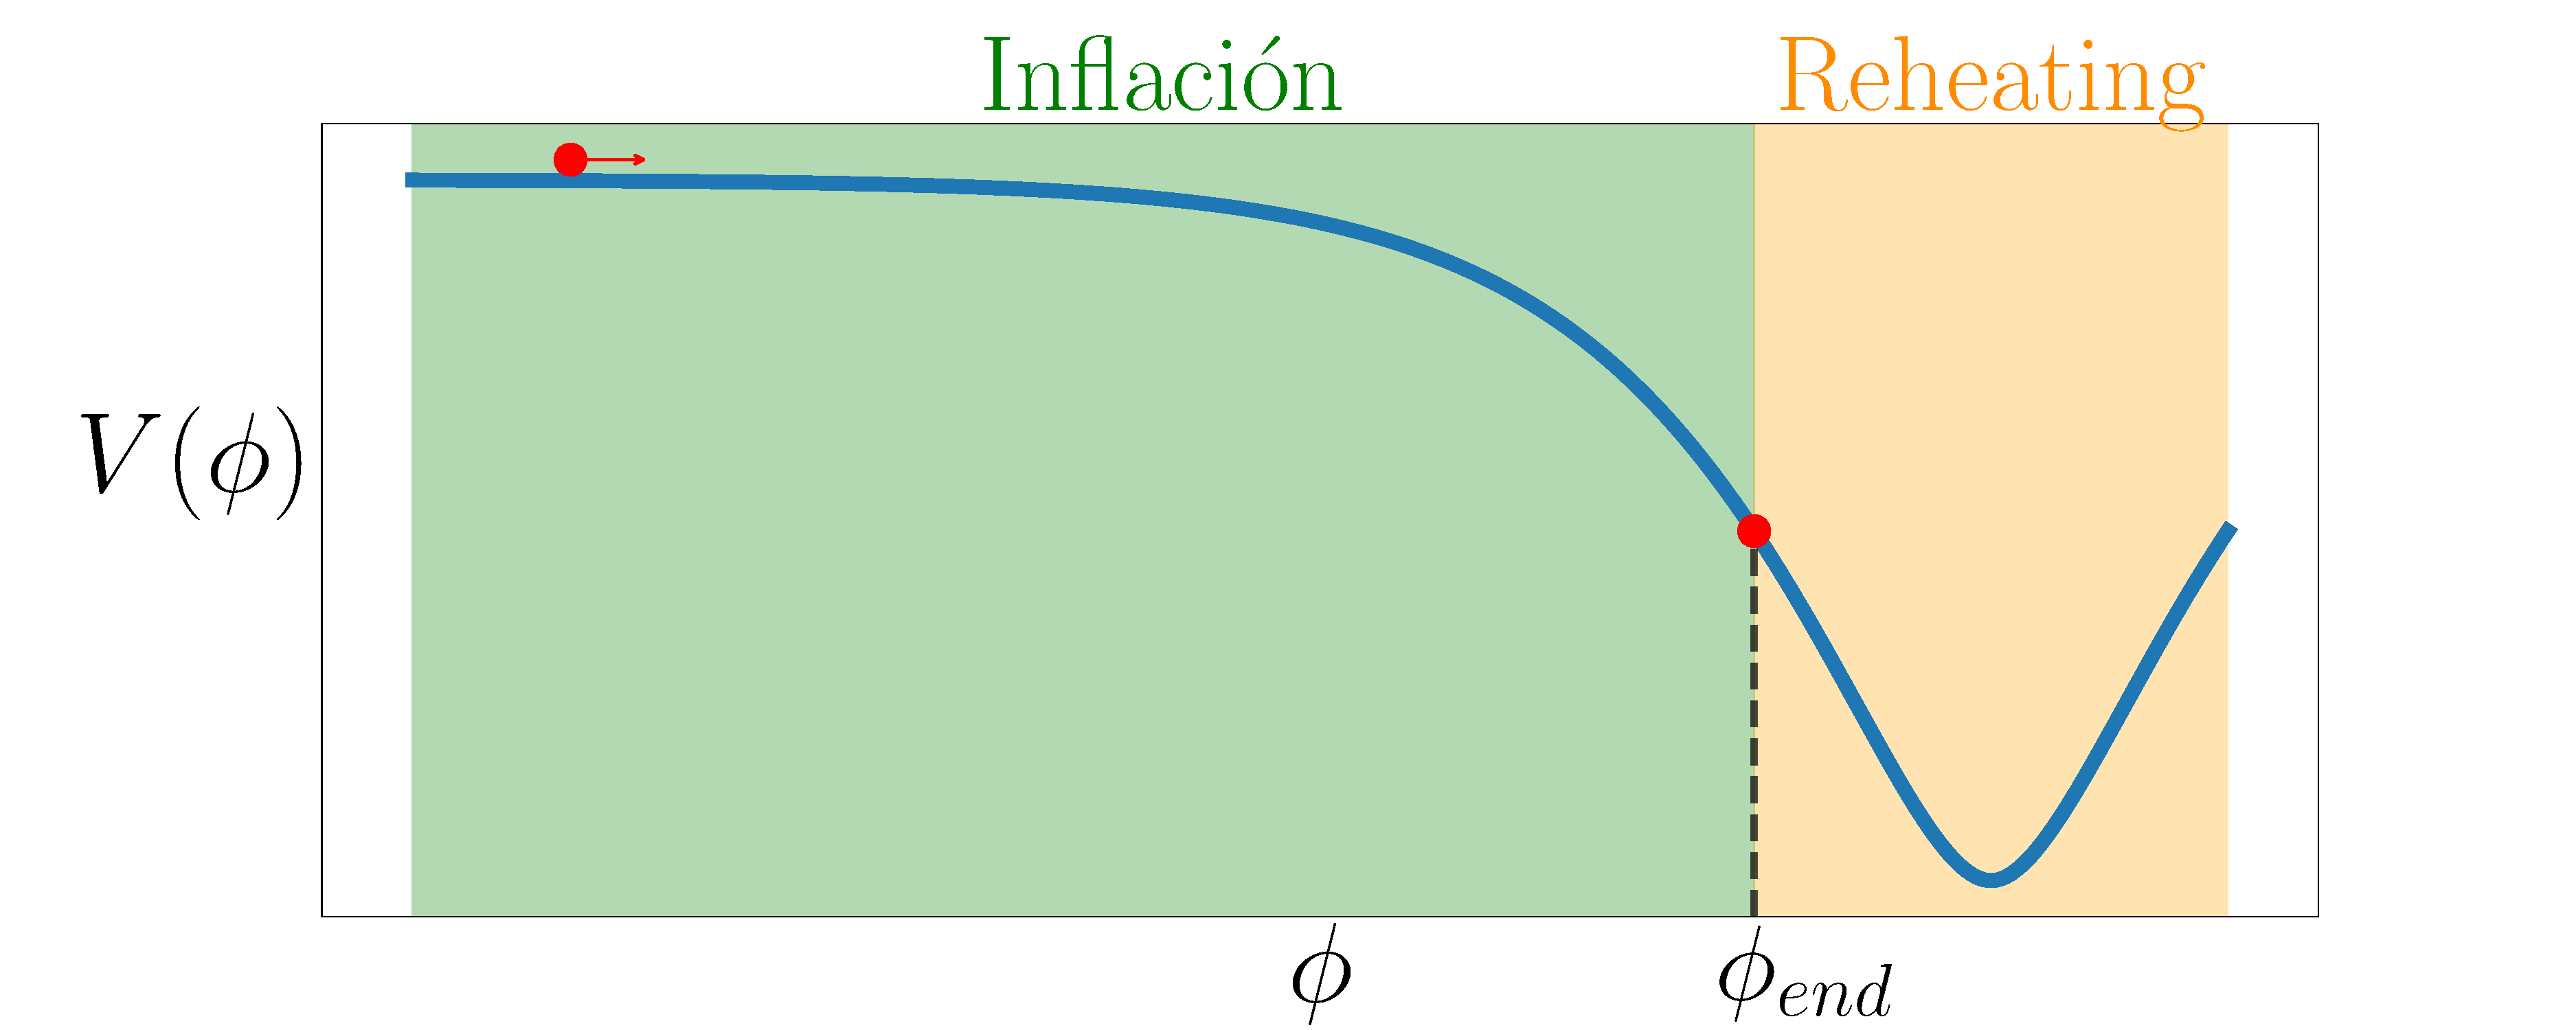
\includegraphics[width = \linewidth]{figures/reheating.pdf}
    \caption{Esquema típico de un potencial inflacionario. A lo largo de la región sombreada en verde ocurre la expansión acelerada, en ésta el inflatón rueda lentamente en dirección al mínimo hasta que su energía cinética resulta comparable con la potencial, dando por finalizada la inflación. Cuando las energías son comparables, se entra en el Recalentamiento marcado como la zona sombreada en naranja, y en esta etapa el inflatón ha perdido suficiente energía debido a la expansión del universo como para no poder regresar a la región plana, por lo que terminará oscilando en torno al mínimo.}
    \label{fig:slowroll}
\end{figure}

Para caracterizar la evolución del parámetro de Hubble  durante la época inflacionaria, se suelen utilizar magnitudes conocidas como parámetros de \textit{slow-roll} tales como
\begin{equation}
    \epsilon = \frac{d}{dt} \left( \frac{1}{H} \right) = \frac{m_p^2}{2} \left[ \frac{V^\prime (\phi)}{V(\phi)} \right]^2,
\end{equation}
\begin{equation}
    \eta = \frac{\ddot{\phi}}{H \dot{\phi}} = \epsilon - m_p^2 \frac{V^{\prime \prime} (\phi)}{V(\phi)},
\end{equation}
siendo $m_p$ la masa de Planck reducida y $H$ el parámetro de Hubble. Estos parámetros son tales que cumplen $\epsilon, \eta \ll 1$ durante Inflación y nos permiten marcar un momento final para esta época como el momento en el cual $\epsilon, \eta \simeq 1$, dando inicio a la época que se conoce como Recalentamiento o \textit{Reheating}. Esto último se encuentra esquematizado en la zona naranja de la Figura \ref{fig:slowroll} dónde $\phi_{end}$ es el valor de la amplitud del campo cuando termina la inflación.

\section{Recalentamiento}\label{sec:reheating}

Una vez finalizada la etapa de Inflación, el universo experimenta una transición conocida como \textit{Recalentamiento} (\textit{Reheating}). Este proceso es el responsable de conectar el estado frío y vacío dejado por la expansión acelerada con el plasma térmico y denso requerido por la teoría del Big Bang caliente, dando lugar posterioriormente a la nucleosíntesis primordial. Un proceso de Recalentamiento completo se compone de tres etapas sucesivas. En primer lugar, la dinámica está dictada por el \textit{Preheating}, una fase violenta donde el inflatón oscila en torno al mínimo de su potencial (tal como se ilustra en la Figura \ref{fig:slowroll}) y transfiere su energía de manera explosiva y no perturbativa hacia otros campos acoplados, típicamente mediante resonancia paramétrica o inestabilidades espinodales \cite{Kofman_1994, Kofman_1997, Amin_2014}. En segundo lugar, se establece un régimen de turbulencia donde las interacciones no lineales re-distribuyen la energía hacia el espectro ultravioleta. Finalmente, el proceso termina con una etapa de termalización, en la cual las interacciones de los campos aseguran el equilibrio cinético y químico de todas las especies.

Para el modelado analítico y numérico de este decaimiento, se asume que el inflatón ($\phi$) decae en nuevos grados de libertad, denominados campos hijos ($\chi$), a través de un término de interacción directo. En el contexto de un estudio no perturbativo, la dinámica del sistema queda determinada por una acción de la forma:
\begin{equation}
    S = \int d^4x \sqrt{-g} \left[ \frac{m_p^2}{2} R - \frac{1}{2} \partial_\mu \phi \partial^\mu \phi - \frac{1}{2} \partial_\mu \chi \partial^\mu \chi - V(\phi) - \mathcal{I} (\phi, \chi)  \right],
\end{equation}
donde $\mathcal{I} (\phi, \chi)$ representa el acoplamiento específico entre los campos. Esta formulación rige la evolución del sistema durante el \textit{Preheating}, dictaminando la tasa de creación de partículas. En el Capítulo \ref{sec:cap3}, se abordará en detalle la dinámica de estos campos a orden lineal para diversos potenciales, y se establecerá su vínculo con la generación de un fondo estocástico de ondas gravitacionales.

Además de la producción lineal de partículas y ondas gravitacionales, la dinámica completa del Recalentamiento involucra una compleja sucesión de fenómenos no lineales que determinan la termalización final del sistema\cite{Elia_2025}. A medida que la densidad de partículas del campo hijo crece exponencialmente, se hace presente la retroacción (\textit{backreaction}) sobre la dinámica del inflatón, este efecto altera la frecuencia de oscilación del condensado y permite la aparición de la dispersión múltiple (\textit{rescattering}), un proceso donde las partículas creadas interactúan entre sí y con el condensado del inflatón. La unión de la retroacción y la dispersión múltiple redistribuye la energía de los modos para aplanar el espectro infrarrojo destruyendo los efectos de amplificación que se obtienen de la resonancia paramétrica. Estos efectos no lineales resultan fundamentales para el equilibrio de la ecuación de estado, ya que fuerzan una rápida transición del universo hacia un estado dominado por radiación. Seguido a ésto, aparece un régimen turbulento, caracterizado por una cascada de energía autosimilar que transporta la densidad de partículas desde escalas infrarrojas hacia el espectro ultravioleta. A medida que la cascada avanza y los números de ocupación decrecen ($n_k \sim 1$), la descripción clásica colapsa y el sistema transiciona hacia un régimen cuántico donde los procesos de dispersión generan un equilibrio cinético. La etapa general concluye con la termalización y el equilibrio químico de todas las especies presentes, estableciendo la temperatura final de Recalentamiento. En la Figura \ref{fig:Reheating_effects} se muestra una cronología esquemática de todos estos fenómenos.

\begin{figure}[htbp]
    \centering
    \begin{tikzpicture}[xscale = 0.75]
        \filldraw[color = esmerald, opacity = 0.5] (-0.5,-3.25) rectangle (4,3.25);
        \filldraw[color = orange, opacity = 0.3] (4,-3.25) rectangle (16,3.25);
        \filldraw[color = violet, opacity = 0.3] (16,-3.25) rectangle (20.5,3.25);
        \draw[->] (-1,0) -- (21,0) node[right] {$t$};

        \draw[->, very thick] (4,3.75) -- (-0.5,3.75);
        \node at (1.75,4.25) {Inflación};
        \draw[decorate,decoration={brace,amplitude=10pt}, very thick] (4,3.55) -- (16,3.55) node[midway,above=10pt]{Reheating};
        \draw[->, very thick] (16,3.75) -- (20.5,3.75);
        \node at (18.25,4.25) {Radiación};

        \draw[->] (4.3,-2.5) -- (4.3,0);
        \draw (4.3,-2.5) -- (4.8,-2.5) node[right] {\small Producción de partículas};
        \draw[->, color = blue, very thick] (6.5,2.5) -- (6.5,0);
        \draw[color = blue, very thick] (6.5,2.5) -- (7,2.5) node[right, color = black] {\textbf{\small{Producción de GW}}};
        \draw[->] (6,-1.75) -- (6,0);
        \draw (6,-1.75) -- (6.5,-1.75) node[right, color = black] {\small Retroacción};
        \draw[->] (7,1.75) -- (7,0);
        \draw (7,1.75) -- (7.5,1.75) node[right, color = black] {\small Dispersión múltiple};
        
        \draw[->, color = red] (8,1) -- (8,0);
        \draw[color = red] (8,1) -- (8.5,1) node[right, color = black] {\small \shortstack{Equilibrio de la\\ecuación de estado}};
        \draw[->] (10,-2) -- (10,0);
        \draw (10,-2) -- (10.5,-2) node[right] {\small Turbulencia};
        \draw[->] (13,-1.5) -- (13,0);
        \draw (13,-1.5) -- (13.5,-1.5) node[right] {\small\shortstack{Régimen\\cuántico}};
        \draw[->] (16,3) -- (16,0);
        \draw (16,3) -- (15.5,3) node[left] {\small{Termalización}};
        \draw[->, color = red] (16,-3) -- (16,0);
        \draw[color = red] (16,-3) -- (15.5,-3) node[left, color = black] {\small Equilibrio químico};

        \draw[->] (17.5,1) -- (17.5,0);
        \draw (17.5,1) -- (18,1) node[right] {\small{BBN}};

        \draw[decorate,decoration={brace,amplitude=10pt,mirror}, very thick] (4,-3.55) -- (10,-3.55) node[midway,below=10pt]{Preheating};
        \draw[decorate,decoration={brace,amplitude=10pt,mirror}, very thick] (12,-3.55) -- (16,-3.55) node[midway,below=10pt]{Equilibración cinética};
    \end{tikzpicture}
    \caption{Línea temporal esquemática de los diversos procesos físicos y dinámicos que ocurren durante el Recalentamiento cosmológico. Adaptado de \cite{Elia_2025}.}
    \label{fig:Reheating_effects}
\end{figure}

La naturaleza de este decaimiento está fuertemente determinada por la forma del potencial inflacionario $V(\phi)$. En la literatura se destacan diversas familias de potenciales, tales como los modelos monomiales $\displaystyle \left( V(\phi) \propto \phi^{2n} \right)$, los modelos de tipo T $\displaystyle \left( V(\phi) \propto \tanh^{2n} (\phi/\mu) \right)$\footnote{Estos modelos forman parte de la clase de \textit{$\alpha$-attractors}, caracterizados por un perfil asintóticamente plano (plateau) a grandes valores del campo y una pendiente pronunciada en las cercanías del mínimo.} y los modelos de tipo E $\displaystyle \left( V(\phi) \propto \left[ 1 - \exp (-\phi/\mu) \right]^{2n} \right)$\footnote{Esta familia engloba, entre otros, al modelo de Starobinsky.}. En el caso particular de los modelos monomiales, tomando el promedio temporal de la ecuación de estado ($P = \omega \rho$) durante las oscilaciones del inflatón en torno al mínimo, se puede demostrar analíticamente que el universo exhibe una ecuación de estado efectiva constante \cite{Turner_1983}:
\begin{equation}\label{eqn:omega_eff}
\left\langle \omega_{eff} \right\rangle = \frac{n - 1}{n + 1}.
\end{equation}
De esta expresión se deduce que para potenciales cuadráticos ($n = 1$), el universo promediado se comporta como si estuviese dominado por materia no relativista ($\omega_{eff} = 0$), mientras que para potenciales cuárticos ($n = 2$), la evolución global emula una dominancia por radiación ($\omega_{eff} = 1/3$). Es importante destacar que este comportamiento analítico es estrictamente válido solo durante las primeras etapas del \textit{Preheating} cuando se tienen oscilaciones coherentes. Posteriormente, la efectos no lineales rompen la coherencia del condensado, forzando invariablemente la transición hacia $\omega_{eff} \to 1/3$, condición necesaria para el acople con la época de dominancia por radiación.

En el marco de este trabajo, se estudiará en detalle cómo el decaimiento del inflatón y la subsecuente producción explosiva de campos hijos excitan perturbaciones tensoriales del espacio-tiempo, dando lugar a la emisión de un fondo estocástico de ondas gravitacionales \cite{Dufaux_2007, Figueroa_2017_GW, Caprini_2020}. El análisis se abordará inicialmente desde un marco teórico a orden perturbativo lineal (Capítulo \ref{sec:cap3}), para luego incorporar rigurosamente la totalidad de los efectos no lineales de las interacciones mediante simulaciones numéricas tridimensionales en redes (\textit{lattice}), empleando el código público \CosmoLattice \cite{Figueroa2021, Figueroa2023, CosmoLatticeNet} (Capítulo \ref{sec:cap4}).
\chapter{Ondas Gravitacionales} \label{sec:cap2}


\chapter{Evolución lineal de los campos} \label{sec:cap3}

\section{Resonancia Paramétrica}

\begin{figure}[htbp]
    \centering
    \begin{subfigure}[t]{0.75\linewidth}
        \centering
        
\includegraphics[width = \linewidth]{figures/background_m2phi2.pdf}
        \subcaption{$m^2 \phi^2$}
    \end{subfigure}
    \begin{subfigure}[b]{0.75\linewidth}
        \centering
        
\includegraphics[width = \linewidth]{figures/Background_lphi4.pdf}
        \subcaption{$\lambda \phi^4$}
    \end{subfigure}
    \caption{}
    \label{fig:Floquet}
\end{figure}


\section{Análisis de Floquet}

\begin{figure}[htbp]
    \centering
    \begin{subfigure}[t]{0.75\linewidth}
        \centering
        
\includegraphics[width = \linewidth]{figures/Floquet_m2phi2.pdf}
        \subcaption{$m^2 \phi^2$}
    \end{subfigure}
    \begin{subfigure}[b]{0.75\linewidth}
        \centering
        
\includegraphics[width = \linewidth]{figures/Floquet_lphi4.pdf}
        \subcaption{$\lambda \phi^4$}
    \end{subfigure}
    \caption{}
    \label{fig:Floquet}
\end{figure}

\begin{figure}[htbp]
    \centering
    \begin{subfigure}[l]{0.45\linewidth}
        \centering
        
\includegraphics[width = \linewidth]{figures/narrow_resonance_m2phi2.pdf}
        \subcaption{Narrow resonance: amplitud}
    \end{subfigure}
    \begin{subfigure}[r]{0.45\linewidth}
        \centering
        
\includegraphics[width = \linewidth]{figures/broad_resonance_m2phi2.pdf}
        \subcaption{Broad resonance: amplitud}
    \end{subfigure}
    \begin{subfigure}[l]{0.45\linewidth}
        \centering
        \includegraphics[width = \linewidth]{figures/nk_Narrow_resonance_m2phi2.pdf}
        \subcaption{Narrow resonance: número de ocupación}
    \end{subfigure}
    \begin{subfigure}[r]{0.45\linewidth}
        \centering
        \includegraphics[width = \linewidth]{figures/nk_Broad_resonance_m2phi2.pdf}
        \subcaption{Broad resonance: número de ocupación}
    \end{subfigure}
    \caption{}
    \label{fig:m2phi2_Resonance}
\end{figure}

\begin{figure}[htbp]
    \centering
    \begin{subfigure}[l]{0.45\linewidth}
        \centering
        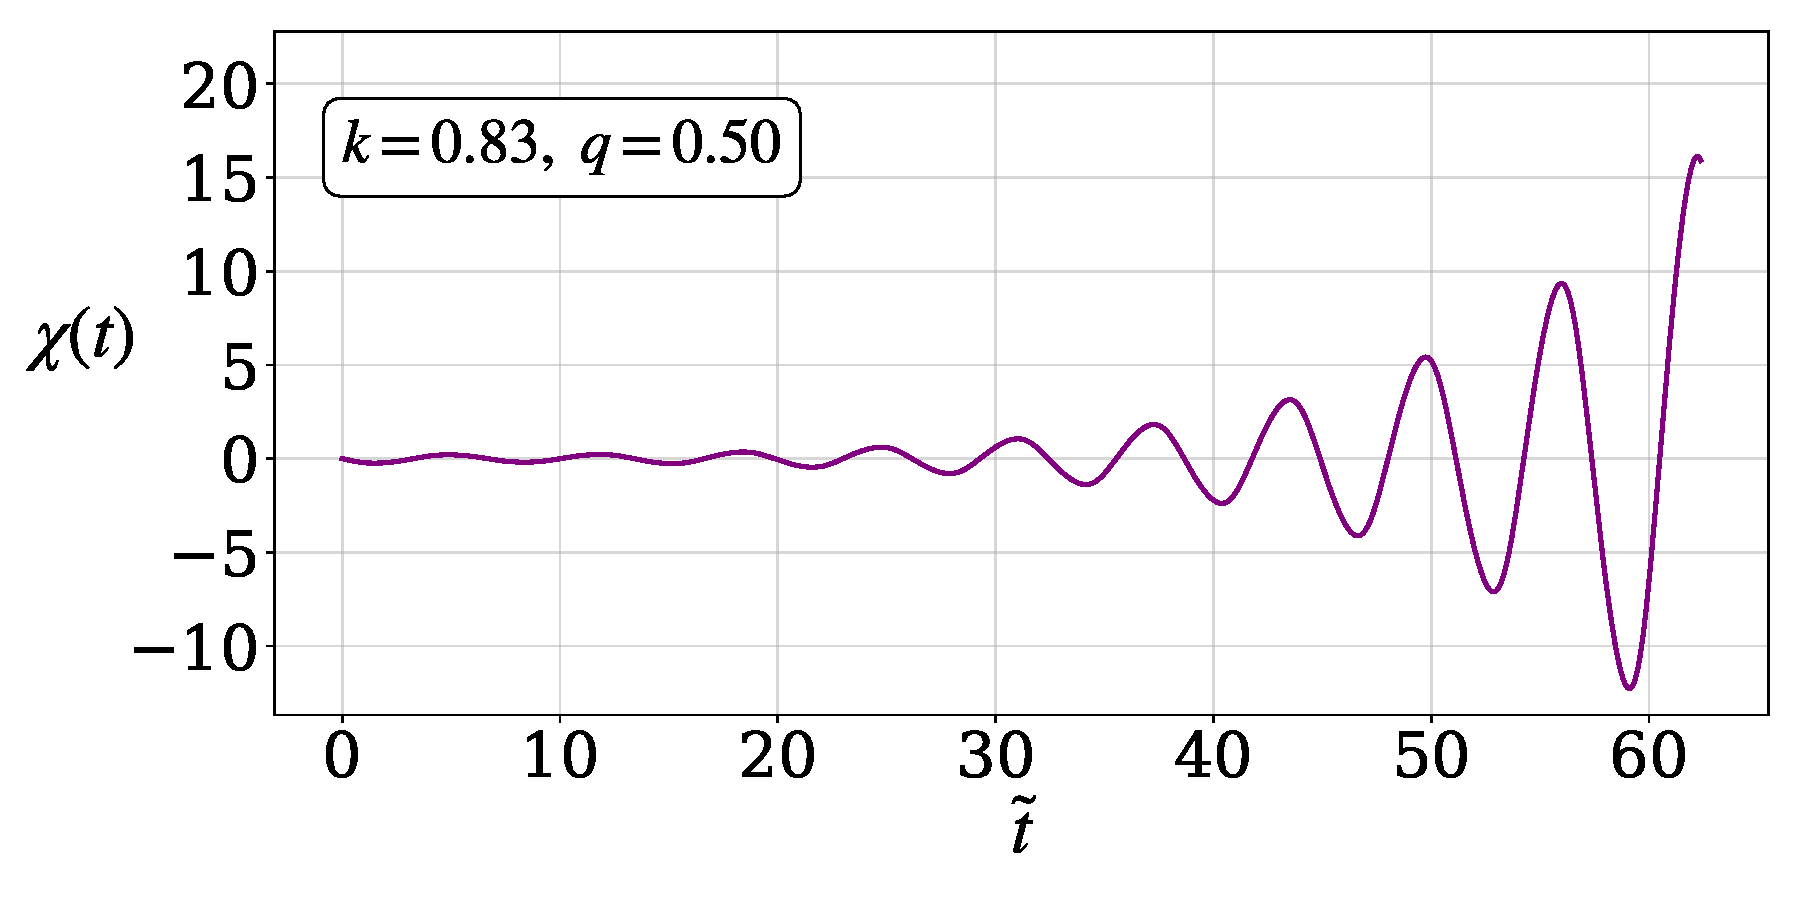
\includegraphics[width = \linewidth]{figures/Narrow_Resonance_lphi4.pdf}
        \subcaption{Narrow resonance: amplitud}
    \end{subfigure}
    \begin{subfigure}[r]{0.45\linewidth}
        \centering
        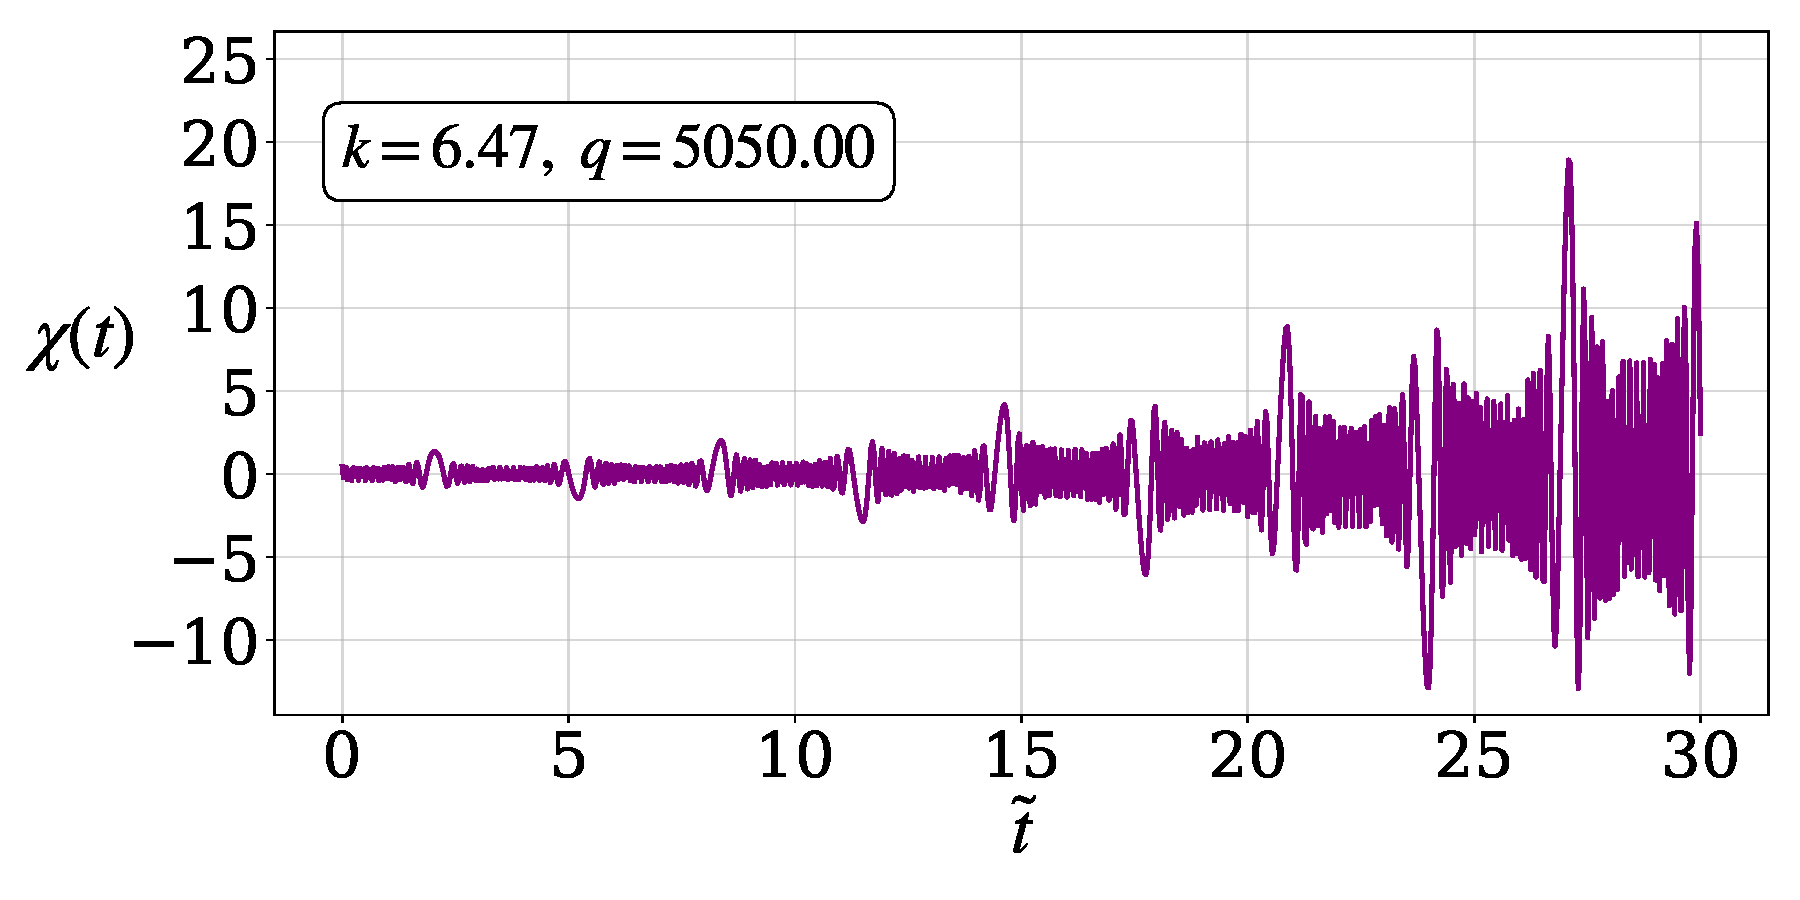
\includegraphics[width = \linewidth]{figures/Broad_Resonance_lphi4.pdf}
        \subcaption{Broad resonance: amplitud}
    \end{subfigure}
    \begin{subfigure}[l]{0.45\linewidth}
        \centering
        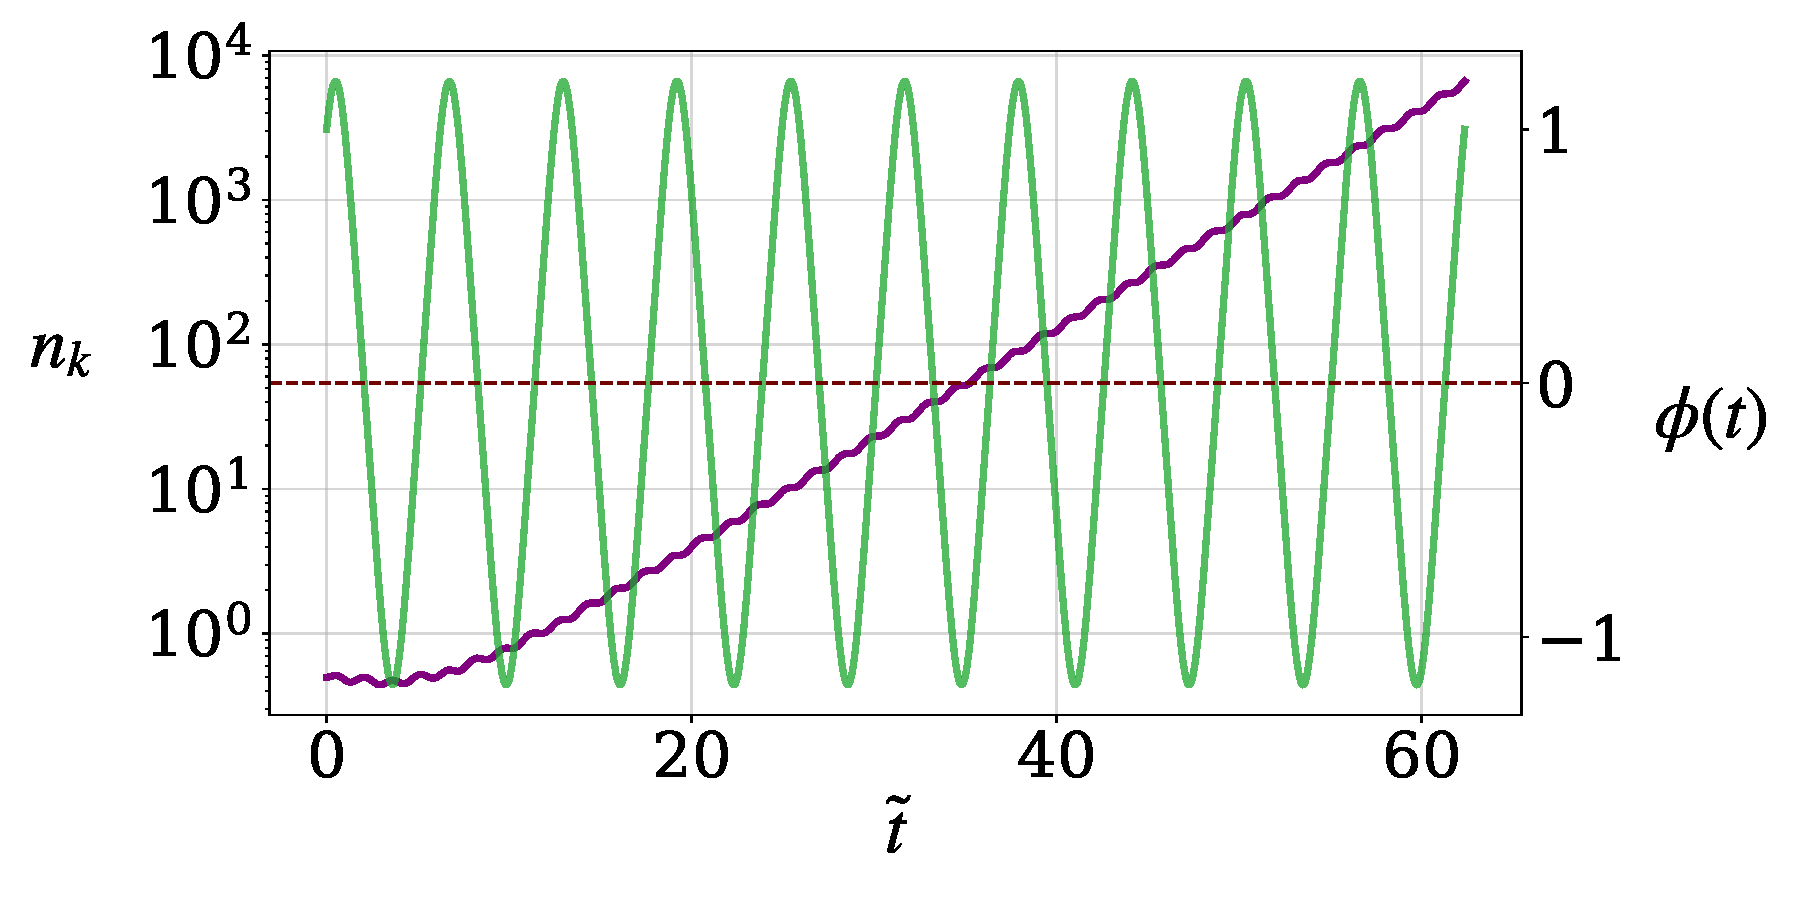
\includegraphics[width = \linewidth]{figures/nk_Narrow_Resonance_lphi4.pdf}
        \subcaption{Narrow resonance: número de ocupación}
    \end{subfigure}
    \begin{subfigure}[r]{0.45\linewidth}
        \centering
        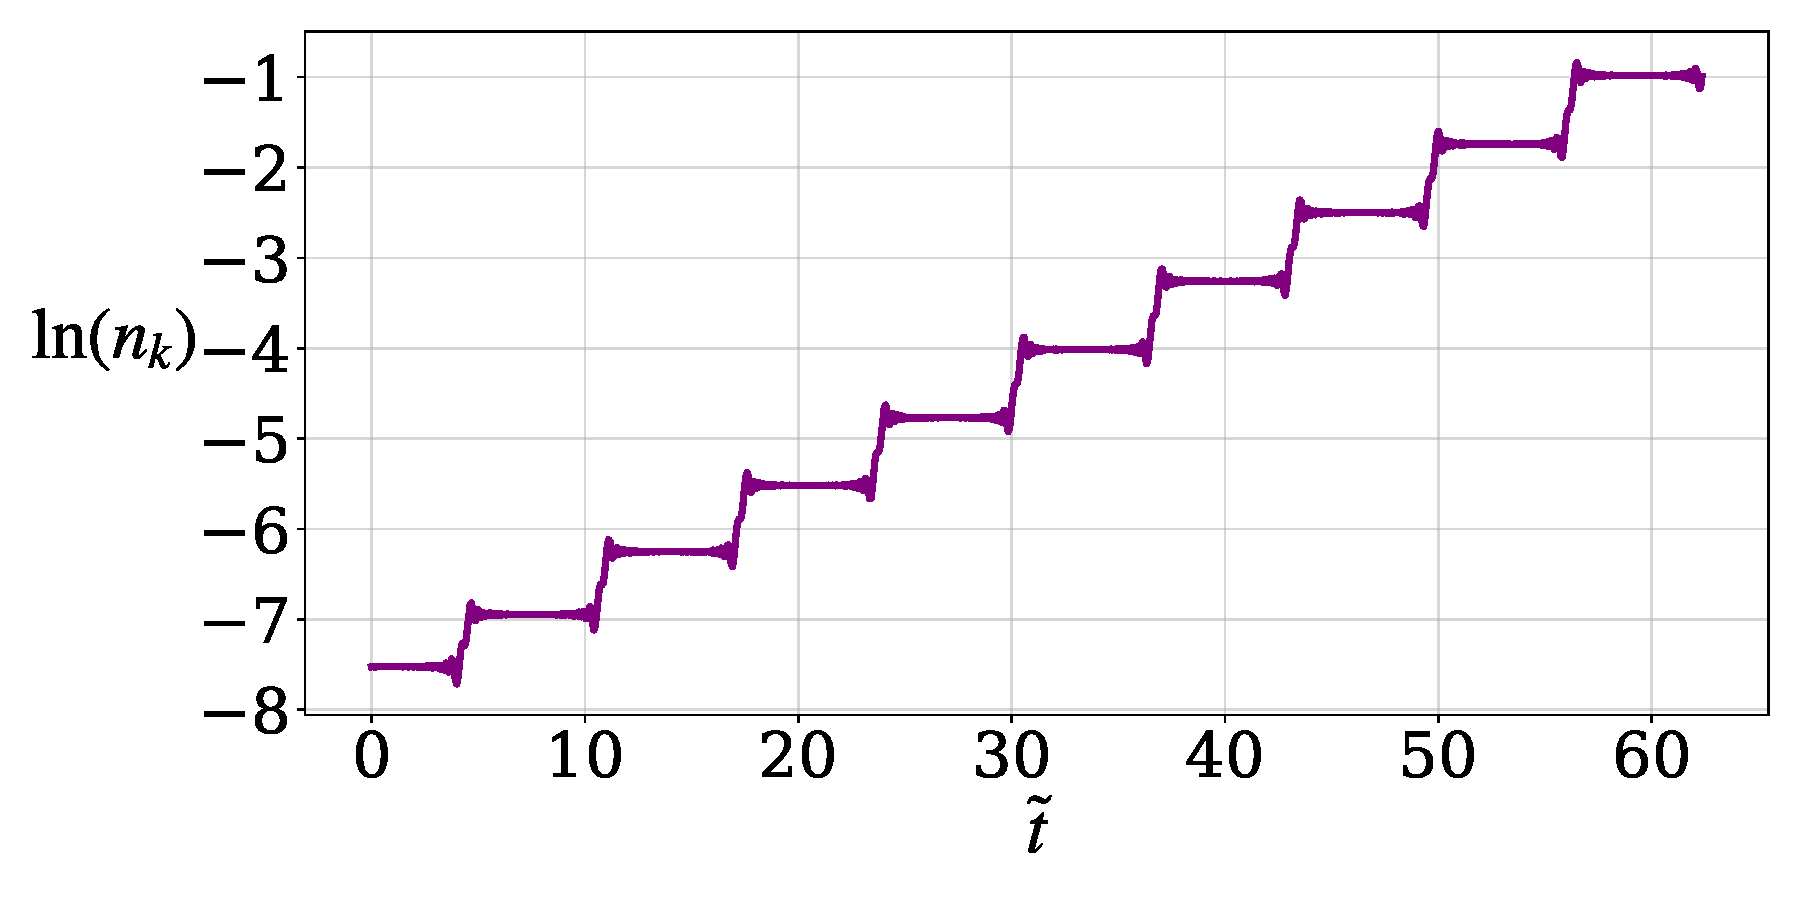
\includegraphics[width = \linewidth]{figures/nk_Broad_Resonance_lphi4.pdf}
        \subcaption{Broad resonance: número de ocupación}
    \end{subfigure}
    \caption{}
    \label{fig:lphi4_Resonance}
\end{figure}

\section{Producción lineal de ondas gravitacionales}

\begin{figure}[htbp]
    \centering
    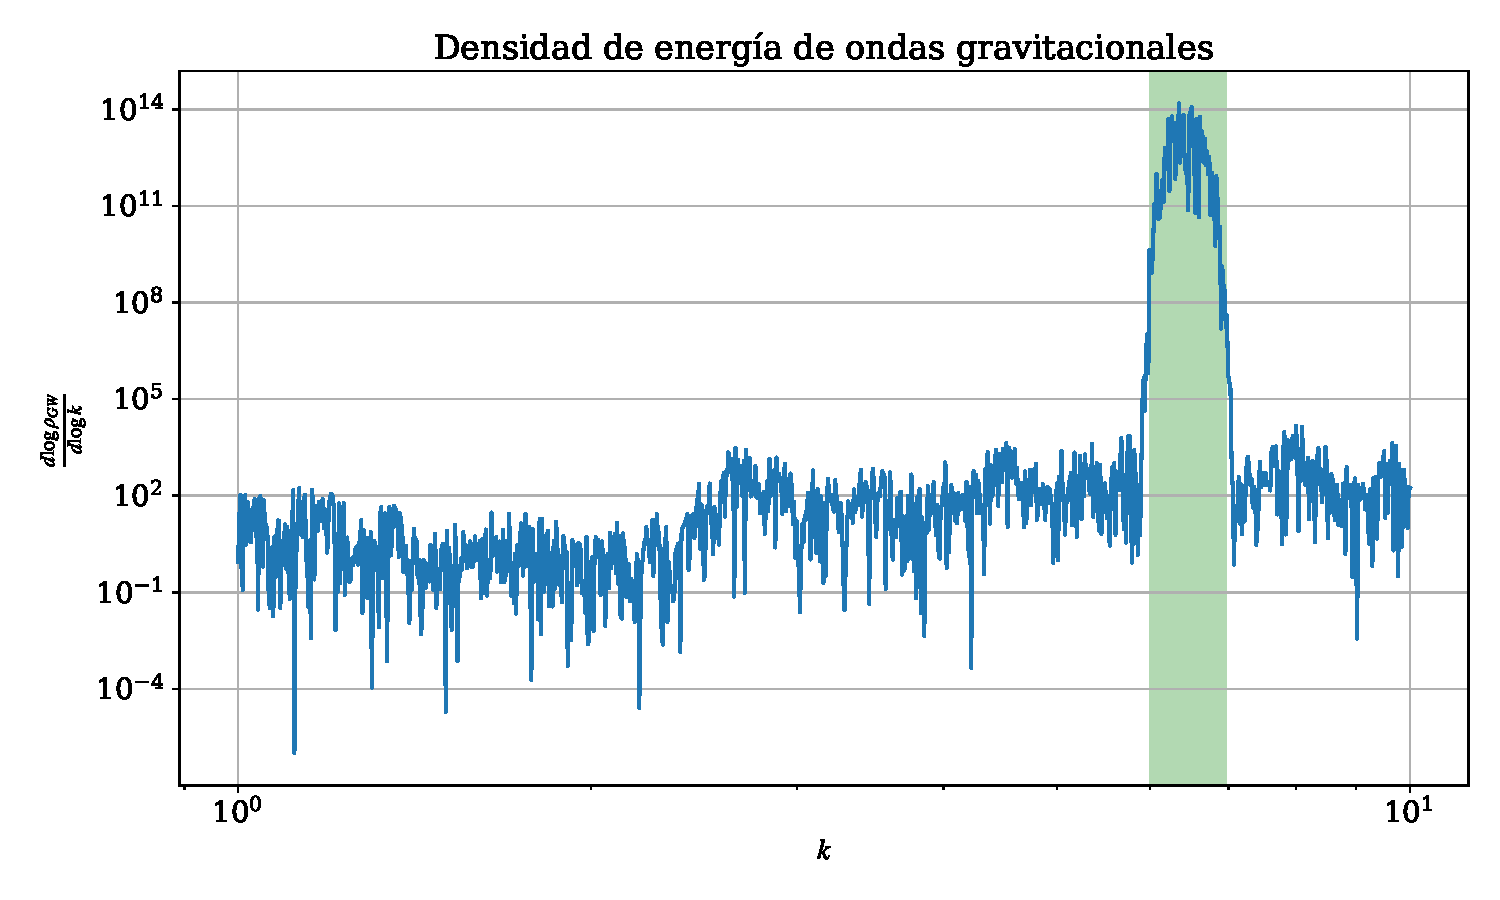
\includegraphics[width = 0.75\linewidth]{figures/rhoGW_lphi4(lineal).pdf}
    \caption{}
    \label{fig:GW_lineal}
\end{figure}
\chapter{\CosmoLattice} \label{sec:cap4}

\section{¿Qué es?}

\section{Estudio del potencial \texorpdfstring{$\lambda \phi^4$}{lambda phi\textasciicircum 4} a orden lineal}

\section{Evolución del background}

\section{Comparación de modelos con \texorpdfstring{$\omega_{eff} = 1/3$}{omega = 1/3}}

\section{Comparación de modelos con \texorpdfstring{$\omega_{eff} = 0$}{omega = 0}}
\chapter{Conclusiones}
\label{cap:conclusiones}

Este trabajo de tesis tuvo como objetivo principal el estudio de la dinámica de los campos escalares durante la época de \textit{Reheating} y la consecuente producción de un Fondo Estocástico de Ondas Gravitacionales (SGWB). A partir del análisis teórico y la implementación de simulaciones numéricas, se han obtenido diversas conclusiones fundamentales que conectan la cosmología primordial con la astrofísica observacional.

En primer lugar, respecto a la dinámica lineal y la resonancia paramétrica, se desarrolló y validó un marco computacional propio a orden lineal para estudiar la evolución del campo inflatón y la subsecuente creación explosiva de partículas durante la etapa de \textit{Preheating}. Esta implementación permitió comprender fenomenológicamente la estructura de las bandas de inestabilidad y los regímenes de resonancia dictados por el análisis de Floquet. Apoyándose en estas herramientas, se analizó el efecto directo de dichas fluctuaciones lineales sobre el tensor de energía-momento. Se corroboró, tanto analítica como numéricamente, que el crecimiento exponencial de los modos escalares actúa como una fuente eficaz para la amplificación del espectro de potencias de las perturbaciones tensoriales.

Para abordar la dinámica en el régimen no perturbativo, se implementó exitosamente el integrador numérico \CosmoLattice. El uso de redes espaciales tridimensionales permitió superar las limitaciones de la teoría lineal, capturando la evolución completa del sistema. Se lograron simular con éxito los efectos de retroacción (\textit{backreaction}), la dispersión no lineal de modos (\textit{rescattering}) y el vaciamiento total del condensado del inflatón, procesos que dictaminan la saturación y la estabilización definitiva de los espectros de ondas gravitacionales.

Mediante estas herramientas, se llevó a cabo una profunda exploración paramétrica, caracterizando el espacio de soluciones para distintas familias de potenciales. Específicamente, se contrastaron modelos de tipo monomial ($m^2\phi^2$, $\lambda\phi^4$) frente a modelos con \textit{plateau} fenomenológicamente favorecidos, como los atractores $\alpha$ (T-models) y el modelo de Starobinsky. Este barrido demostró de forma concluyente cómo la pendiente del pozo de potencial y la escala de acoplamiento modifican drásticamente la forma del espectro, la frecuencia pico y la amplitud general de la energía tensorial inyectada.

Finalmente, para establecer la sensibilidad observacional del modelo, se reescalaron los espectros teóricos proyectándolos al \textit{strain} característico ($h_c$) observable en la actualidad. Al confrontarlos con las curvas de sensibilidad de arreglos de púlsares (PTA), interferómetros láser y cavidades resonantes electromagnéticas (EMRC), se concluyó que estos últimos experimentos de ultra-alta frecuencia representan la vía más prometedora para la detección de este tipo de señales. Además, se demostró que el paso al espacio del \textit{strain} introduce una ruptura de degeneración para los modelos de tipo materia ($\omega_{eff}=0$): mientras que la densidad de energía $\Omega_{GW}$ de estos modelos resulta virtualmente idéntica a tiempos largos, la dependencia del \textit{strain} con la inversa de la frecuencia magnifica su separación. Esto evidencia que el SGWB posee el poder resolutivo necesario para discriminar empíricamente entre los distintos modelos inflacionarios subyacentes.

\section*{Perspectivas futuras}

Como extensión de este trabajo, resulta de particular interés abordar el estudio de escenarios más complejos que incorporen campos vectoriales de gauge (U(1) o SU(2)) en las simulaciones de \CosmoLattice, con el fin de evaluar cómo las interacciones de norma modifican la eficiencia en la transferencia de energía y la consecuente firma gravitacional. Asimismo, sería valioso ampliar el análisis espectral considerando familias de potenciales polinomiales, tal como se ha propuesto recientemente en la literatura para dinámicas de tipo \textit{hilltop} \cite{Das_2025}. Finalmente, otra dirección prometedora consistiría en enmarcar este estudio dentro de teorías de gravedad modificada, analizando la dinámica y la producción de ondas gravitacionales en escenarios donde el acoplamiento de los campos de materia con la gravedad es no mínimo.

% --- BIBLIOGRAFÍA ---
\bibliographystyle{apalike}
\bibliography{references}

% --- APÉNDICES ---
\appendix
\appendix
\chapter{Produción lineal de ondas gravitacionales} \label{sec:apexA}

\newpage

\chapter{Condiciones iniciales \CosmoLattice} \label{sec:apexB}

A la hora de querer calcular las condiciones iniciales para el campo inflatón al entrar en \textit{reheating} se utilizó el parámetro $\epsilon$ de \textit{slow-roll} definido como

\begin{equation}
    \epsilon = \frac{m_p^2}{2} \left[ \frac{V^{\prime} \left( \phi \right)}{V \left( \phi \right)} \right]^2,
\end{equation}

\noindent
dado que considerar $\epsilon \simeq 1$ denota el final de la etapa inflacionaria. A su vez, para calular la velocidad de los campos se pidió que la energía cinética del campo sea comparable con la energía potencial, dando como condición\footnote{El signo negativo en la velocidad está dado ya que se espera que el campo decaiga y por tanto su amplitud debe disminuir.}

\vspace{-0.7cm}

\begin{equation}
    \dot{\phi}_0 = - \sqrt{2 V \left( \phi_0 \right)}. 
\end{equation}

\vspace{-0.25cm}

\noindent
De este modo, abajo se desarrollan las cuentas realizadas para calcular las condiciones iniciales para cada modelo.

\begin{itemize}
    \item $\displaystyle V(\phi) = \frac{1}{2} m^2 \phi^2$
    
    Para la amplitud inicial se tiene

    \vspace{-0.9cm}

    \begin{equation*}
        \begin{split}
            \frac{m_p^2}{2} \left( \frac{m^2 \phi_0}{\frac{1}{2} m^2 \phi_0^2} \right)^2 &= 1\\
            \frac{2 m_p^2}{\phi_0^2} &= 1
        \end{split}
    \end{equation*}

    \vspace{-0.5cm}

    \begin{equation}
        \phi_0^{m} = \sqrt{2} m_p
    \end{equation}

    Y la condición para la velocidad inicial sería

    \vspace{-1cm}

    \begin{equation*}
        \begin{split}
            \dot{\phi}_0 &= - \sqrt{m^2 \phi_0^2}
        \end{split}
    \end{equation*}

    \vspace{-1cm}

    \begin{equation}
        \dot{\phi}_0^{m} = - \sqrt{2} m m_p
    \end{equation}

    \item $\displaystyle V(\phi) = \frac{\Lambda^4}{2} \tanh^2 \left( \frac{\phi}{M} \right)$
    
    Para la amplitud inicial se tiene

    \vspace{-0.9cm}

    \begin{equation*}
        \begin{split}
            \frac{m_p^2}{2} \left[ \frac{\frac{\Lambda^4}{M} \tanh \left( \frac{\phi_0}{M} \right) \text{sech}^2 \left( \frac{\phi_0}{M} \right)}{\frac{1}{2} \Lambda^4 \tanh^2 \left( \frac{\phi_0}{M} \right)} \right]^2 &= 1\\
            \frac{m_p^2}{2} \left[ \frac{2 \text{sech}^2 \left( \frac{\phi_0}{M} \right)}{M \tanh \left( \frac{\phi_0}{M} \right)} \right]^2 &= 1\\
            \frac{m_p^2}{2} \left[ \frac{2}{M \sinh \left( \frac{\phi_0}{M} \right) \cosh \left( \frac{\phi_0}{M} \right)} \right]^2 &= 1\\
            \frac{m_p^2}{2} \left[ \frac{4}{M \sinh \left( 2 \frac{\phi_0}{M} \right)} \right]^2 &= 1\\
            \frac{8 m_p^2}{M^2 \sinh^2 \left( 2 \frac{\phi_0}{M} \right)} &= 1\\
            \sinh^2 \left( 2 \frac{\phi_0}{M} \right) &= 8 \left( \frac{m_p}{M} \right)^2\\
            2 \frac{\phi_0}{M} &= \text{arcsinh} \left( 2 \sqrt{2} \frac{m_p}{M} \right)
        \end{split}
    \end{equation*}

    \vspace{-0.5cm}

    \begin{equation}
        \phi_0^{t2} = \frac{M}{2} \text{arcsinh} \left( 2 \sqrt{2} \frac{m_p}{M} \right)
    \end{equation}

    Y la condición para la velocidad inicial sería

    \vspace{-1cm}

    \begin{equation*}
        \begin{split}
            \dot{\phi}_0 &= -\sqrt{\Lambda^4 \tanh^2 \left( \frac{\phi_0}{M} \right)}\\
            \dot{\phi}_0 &= - \Lambda^2 \tanh \left( \frac{\phi_0}{M} \right)
        \end{split}
    \end{equation*}

    \vspace{-1cm}

    \begin{equation}
        \dot{\phi}_0^{t2} = - \Lambda^2 \tanh \left[ \frac{1}{2} \text{arcsinh} \left( 2 \sqrt{2} \frac{m_p}{M} \right) \right]
    \end{equation}

    \newpage

    \item $\displaystyle V(\phi) = \frac{\Lambda^4}{2} \left[ 1 - \exp \left( \frac{\phi}{M} \right) \right]^2$ (Starobinsky)
    
    Para la amplitud inicial se tiene

    \vspace{-0.9cm}

    \begin{equation*}
        \begin{split}
            \frac{m_p^2}{2} \left\{ \frac{\frac{\Lambda^4}{M} \left[ 1 - \exp \left( - \frac{\phi_0}{M} \right) \right] \exp \left( - \frac{\phi_0}{M} \right)}{\frac{1}{2} \Lambda^4 \left[ 1 - \exp \left(- \frac{\phi_0}{M} \right) \right]^2} \right\}^2 &= 1\\
            \frac{m_p^2}{2} \left\{ \frac{2 \exp \left(- \frac{\phi_0}{M} \right)}{M \left[ 1 - \exp \left(- \frac{\phi_0}{M} \right) \right]} \right\}^2 &= 1\\
            \frac{m_p^2}{2} \left\{ \frac{2}{M \left[ \exp \left(\frac{\phi_0}{M} \right) - 1 \right]} \right\}^2 &= 1\\
            \frac{2 m_p^2}{M^2 \left[ \exp \left(\frac{\phi_0}{M} \right) - 1 \right]^2} &= 1\\ 
            \left[ \exp \left(\frac{\phi_0}{M} \right) - 1 \right]^2 &= 2 \left( \frac{m_p}{M} \right)^2\\
            \exp \left( \frac{\phi_0}{M} \right) &= \sqrt{2} \frac{m_p}{M} + 1\\
            \frac{\phi_0}{M} &= \ln \left( \sqrt{2} \frac{m_p}{M} + 1 \right) 
        \end{split}
    \end{equation*}

    \vspace{-0.5cm}

    \begin{equation}
        \phi_0^{s} = M \ln \left( \sqrt{2} \frac{m_p}{M} + 1 \right)
    \end{equation}

    Y la condición para la velocidad inicial sería

    \vspace{-1cm}

    \begin{equation*}
        \begin{split}
            \dot{\phi}_0 &= -\sqrt{\Lambda^4 \left[ 1 - \exp \left(- \frac{\phi_0}{M} \right) \right]^2}\\
            \dot{\phi}_0 &= -\Lambda^2 \left[ 1 - \exp \left( - \frac{\phi_0}{M} \right) \right]\\
            \dot{\phi}_0 &= -\Lambda^2 \left\{ 1 - \exp \left[ - \ln \left( \sqrt{2} \frac{m_p}{M} + 1 \right) \right] \right\}\\
            \dot{\phi}_0 &= -\Lambda^2 \left( 1 - \frac{1}{\sqrt{2} \frac{m_p}{M} + 1} \right)\\
            \dot{\phi}_0 &= -\Lambda^2 \frac{\sqrt{2} \frac{m_p}{M}}{\sqrt{2} \frac{m_p}{M} + 1}
        \end{split}
    \end{equation*}

    \vspace{-1cm}

    \begin{equation}
        \dot{\phi}_0^{s} = - \frac{\sqrt{2} \Lambda^2 m_p }{\sqrt{2} m_p + M}
    \end{equation}

    \newpage

    \item $\displaystyle V(\phi) = \frac{1}{4} \lambda \phi^4$
    
    Para la amplitud inicial se tiene

    \vspace{-0.9cm}

    \begin{equation*}
        \begin{split}
            \frac{m_p^2}{2} \left( \frac{\lambda \phi_0^3}{\frac{1}{4} \lambda \phi_0^4} \right)^2 &= 1\\
            \frac{8 m_p^2}{\phi_0^2} &= 1 
        \end{split}
    \end{equation*}

    \vspace{-0.5cm}

    \begin{equation}
        \phi_0^{\lambda} = M \ln \left( \sqrt{2} \frac{m_p}{M} + 1 \right)
    \end{equation}

    Y la condición para la velocidad inicial sería

    \vspace{-1cm}

    \begin{equation*}
        \begin{split}
            \dot{\phi}_0 &= - \sqrt{\frac{1}{2} \lambda \phi_0^4}\\
        \end{split}
    \end{equation*}

    \vspace{-1cm}

    \begin{equation}
        \dot{\phi}_0^{\lambda} = - 4 \sqrt{2 \lambda} m_p^2
    \end{equation}

    \item $\displaystyle V(\phi) = \frac{\Lambda^4}{4} \tanh^4 \left( \frac{\phi}{M} \right)$
    
    Para la amplitud inicial se tiene

    \vspace{-0.9cm}

    \begin{equation*}
        \begin{split}
            \frac{m_p^2}{2} \left[ \frac{\frac{\Lambda^4}{M} \tanh^3 \left( \frac{\phi_0}{M} \right) \text{sech}^2 \left( \frac{\phi_0}{M} \right)}{\frac{1}{4} \Lambda^4 \tanh^4 \left( \frac{\phi_0}{M} \right)} \right]^2 &= 1\\
            \frac{m_p^2}{2} \left[ \frac{8}{M \sinh \left( 2 \frac{\phi_0}{M} \right)} \right]^2 &= 1\\
            \frac{32 m_p^2}{M^2 \sinh^2 \left( 2 \frac{\phi_0}{M} \right)} &= 1\\
        \end{split}
    \end{equation*}

    \vspace{-0.5cm}

    \begin{equation}
        \phi_0^{t4} = \frac{M}{2} \text{arcsinh} \left( 4 \sqrt{2} \frac{m_p}{M} \right)
    \end{equation}

    Y la condición para la velocidad inicial sería

    \vspace{-1cm}

    \begin{equation*}
        \begin{split}
            \dot{\phi}_0 &= -\sqrt{\frac{1}{2} \Lambda^4 \tanh^4 \left( \frac{\phi_0}{M} \right)}\\
        \end{split}
    \end{equation*}

    \vspace{-1cm}

    \begin{equation}
        \dot{\phi}_0^{t4} = - \sqrt{\frac{1}{2}} \Lambda^2 \tanh^2 \left[ \frac{1}{2} \text{arcsinh} \left( 4 \sqrt{2} \frac{m_p}{M} \right) \right]
    \end{equation}
\end{itemize}

\newpage

\chapter{Ánalisis en la estabilidad de modelos en \CosmoLattice} \label{sec:apexC}

% Marcador para el total de páginas arábigas
\label{ultimaPagina}

% --- PÁGINA FINAL (LICENCIA) ---
\newpage
\section*{}
\thispagestyle{empty} 

\begin{flushright}
\null\vspace{\stretch{1}}
\begin{center}Tesis disponible bajo Licencia Creative Commons, Atribución – No Comercial – Compartir Igual (by-nc-sa) 2.5 Argentina\\
Buenos Aires, 2026
\end{center}
\vspace{\stretch{4}}\null
\end{flushright}

\end{document}